\chapter{Discussions}\label{discuss}

\section{Performance Quantization}

To further quantify the performance of PoLaR BEAR, the average deviations in the detection parameters were observed. Table \ref{tab:frbdev} and \ref{tab:fakedev} shows the average deviations in the detections for PoLaR BEAR and BEAR for both real FRB data and fake FRB data respectively. For real FRB data, it can be see that PoLaR BEAR performs significantly better than BEAR for detection DM and W, and only slightly worse for detection SNR. For fake FRB data, it can be see that PoLaR BEAR performs slightly worse than BEAR for detection DM and SNR, and slightly better for detection SNR. Therefore, it can be confirmed that PoLaR BEAR performs comparably well with BEAR.

\begin{table}
\centering
\def\arraystretch{1.25}
\caption[Average deviations in the detection parameters for real FRB data]{Average deviations in the detection parameters using PoLaR BEAR and BEAR for real FRB data.}
\begin{tabular}{cccc}
\hline
Parameter & DM ($\cmp$) & W (ms) & SNR\\
\hline
PoLaR BEAR & 2.9953  & 1.6203   & 10.4972 \\
BEAR       & 45.9694 & 116.6431 & 9.9726  \\
\hline
\end{tabular}
\label{tab:frbdev}
\end{table}
\begin{table}
\centering
\def\arraystretch{1.25}
\caption[Average deviations in the detection parameters for fake FRB data]{Average deviations in the detection parameters using PoLaR BEAR and BEAR for fake FRB data.}
\begin{tabular}{cccc}
\hline
Parameter & DM ($\cmp$) & W (ms) & SNR\\
\hline
PoLaR BEAR & 2.0530   & 0.4282  & 5.0371 \\
BEAR       & 1.7404   & 0.5089  & 3.8685  \\
\hline
\end{tabular}
\label{tab:fakedev}
\end{table}

There was also one significant outlier for detections in BEAR that were not present in PoLaR BEAR, namely FRB 010724. BEAR detected a DM of $930.767 \cmp$, which is $555.767 \cmp$ away from the actual value, whereas PoLaR BEAR reported a DM of $374 \cmp$. BEAR also detected a W of $1529\,\text{ms}$, which is $1509\,\text{ms}$ away from the actual value, whereas PoLaR BEAR reported a W of $24\,\text{ms}$. Figure \ref{fig:frb010724} shows the candidate plot of the detection in PoLaR BEAR. A large decrease in flux after the burst can be seen due to saturation of the receiver, causing the inaccurate detection in BEAR. 

\begin{sidewaysfigure}
    \centering
    \includegraphics[width=0.9\textwidth]{Images/FRB010724.jpeg}
    \caption{PoLaR BEAR candidate output for FRB 010724.}
    \label{fig:frb010724}
\end{sidewaysfigure}

\section{Underestimation of SNR}

In general, the SNRs are detected by PoLaR BEAR and BEAR can be seen to be slightly lower than that of the true values. This is expected as inaccurate DM and W values when performing the calculation for $S$ would result in lower $S$ values, and consequently lower detected SNR. For a DM offset of $\delta$DM, the ratio between the SNR detected and the true SNR is \cite{Cordes2003}
\begin{equation}
    \frac{\text{SNR}}{\text{SNR}_0} = \frac{\sqrt{\pi}}{2} \zeta^{-1} \text{erf }\zeta
\end{equation}
where $\text{SNR}_0$ is the true SNR if the dedispersion is perform at the true DM. $\zeta$ is the ratio between the time delay caused by the DM offset and pulse width given by
\begin{equation}
    \zeta = 6.91 \times 10^{-3} \delta \text{DM} \frac{\Delta\nu_{\text{MHz}}}{W_{\text{ms}}\nu^3_{\text{GHz}}}
\end{equation}
As for a W offset of $\delta W$, the SNR ratio becomes \cite{Men2019}
\begin{equation}
    \frac{\text{SNR}}{\text{SNR}_0} = \begin{cases}\frac{W}{W+\delta W}, & \text{for }\delta W\geq 0, \\ \frac{W+\delta W}{W}, & \text{for }\delta W < 0\end{cases}
\end{equation}
For any non-zero offset in DM and W, both cases results a lower detection SNR compared to SNR$_0$, shown in Figure \ref{fig:snrdev}. 

\begin{figure}
    \centering
    \begin{minipage}{0.5\textwidth}
    \includegraphics[width=\textwidth]{Graphs/snrdm.eps}
    \end{minipage}%
    \begin{minipage}{0.5\textwidth}
    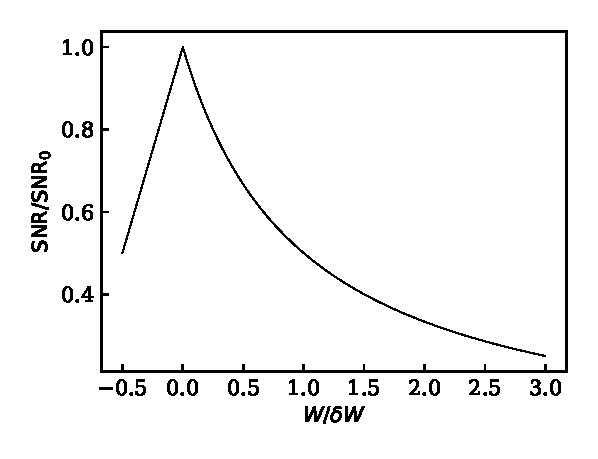
\includegraphics[width=\textwidth]{Graphs/snrw.eps}
    \end{minipage}
    \caption[SNR deviation due to DM and W offset]{Graph of SNR deviation due to DM offset i.e. $\zeta \propto \delta\text{DM}$ (left), and due to W offset i.e. $\delta W/W$ (right). Detected SNR decreases for any non-zero $\delta\text{DM}$ and $\delta W/W$.}
    \label{fig:snrdev}
\end{figure}

\section{Differences between PoLaR BEAR and BEAR}

Other than the differences between Python and C++, there are two main differences between PoLaR BEAR and BEAR. The first is the division of trial DMs. In BEAR, subband dedispersion is use to improve its efficacy \cite{Barsdell2012}. Subband dedispersion is an approximation approach in reducing the computation cost of dedispersion. The process involves splitting up the DM range into several subranges, each centered around a nominal DM value. The frequency channels are also partitioned into subbands. The delays for every nominal DMs are subtracted from the subbands, resulting in partially dedispersed subbands. The data is then passed through the usual dedispersion at the remaining DMs. This results in a trial DM array with differing increments depending on the nominal DM, usually larger increments at higher DMs, as shown in Table \ref{tab:subband} \cite{Magro2011}.

\begin{table}[h]
    \def\arraystretch{1.25}
    \caption[Example of a subband dedispersion plan]{Example of a subband dedispersion plan for a pulsar survey. $\Delta$Sub$_{\text{DM}}$ refers to the DM step between two successive nomial DM values, $\Delta$DM is the finer step used for creating the dedispersed time series around a particular nominal DM value.}
    \centering
    \begin{tabular}{ccccc}
        \hline
        Pass & Low DM & High DM & $\Delta$DM & $\Delta$Sub$_{\text{DM}}$ \\
        & ($\cmp$) & ($\cmp$) & ($\cmp$) & ($\cmp$) \\
        \hline
        1 & 0.00 & 53.46 & 0.03 & 0.66 \\
        2 & 53.46 & 88.26 & 0.05 & 1.2 \\
        3 & 88.26 & 150.66 & 0.10 & 2.4 \\
        \hline
    \end{tabular}
    \label{tab:subband}
\end{table}

However, in PoLaR BEAR, I opted to set the DM range and a single increment in the beginning (usually from 1 to 2000 $\cmp$ with increments of 1 $\cmp$) and use the usual brute force dedispersion. This is because the program is aimed to allow for an easier understanding in FRB detection instead of performance. 

Another difference is in the definition of the detection time or also known as the pulse epoch, $t_0$. In BEAR, $t_0$ is defined to be the beginning of the pulse, allowing it to utilize efficient looping methods for the calculation of $S$. However in PoLaR BEAR, $t_0$ is defined to be in the middle of the pulse, allowing the usage of convolution in the program which follows the usual Python style. 

\section{GPU Dedispersion}

As stated in \citeNP{Magro2011}, graphics processing unit or GPU computation can also speed up dedispersion to improve real time detection of radio transients. Using NVIDIA's CUDA cores, dedispersion can be parallelized over many GPU threads, simultaneously operating on many different DMs. Tests have shown that GPUs speed up dedispersion by 50 to 200 times \cite{Magro2011} or at least by 9 times \cite{Barsdell2012} when compared to single-threaded CPU implementation. This is applied in many FRB searches e.g. AMBER used on the Westerbork Telescope \cite{Sclocco2020} and the Medicina BEST-2 transient search pipeline \cite{MAGRO2013}. 

In Python, two packages allows python to utilize GPU to speed up numpy functions, namely \texttt{CuPy} and \texttt{Numba}. In this case, \texttt{CuPy} was used as it is a more complete reimplementation of \texttt{Numpy} using the GPU, compared to \texttt{Numba} where custom algorithms tailored to its format is required \cite{Okuta2017}.

To test the performance increase of GPU dedispersion in this case, the data was generated using the same method with the same properties as for fake FRB, with varying observation times i.e. 0.125, 0.25, 0.5, 1, 2, and 5 minutes, and varying number of frequency channels i.e. 128, 256, 512, and 1024 frequency channels. The data is also downsampled by 20 to reduce computation time. The data is then dedispersed using both brute force dedispersion with \texttt{numpy.roll} and a modified dedispersion with \texttt{cupy.roll} at a single DM (1000$\cmp$), as dedispersion at different DMs should not affect the performance significantly. Note that the GPU used here is the GTX 1660 Ti, with 1536 CUDA cores rated at a maximum of 169.9 GFLOPS, and 6 GB of memory. 

Figure \ref{fig:gpu} shows the graph of the speed-up factor of GPU dedispersion compared to the brute force CPU implementation for different data length/observation time, as well as at different number of frequency channels. The speed-up factor can be seen to increase with observation times up to a factor of 8, but shorter observation times result in speed-up factors of less than one i.e. GPU dedispersion slower than CPU implementation, which could be due to the memory transfer latency between the RAM and the GPU memory. Therefore, implementation of GPU dedispersion in PoLaR BEAR using \texttt{CuPy} can be beneficial to improve its performance. Note that the benefits may scale further at larger observation time, but requires a much larger amount of GPU memory, which is the reason that the tests was only done for data up to 5 minutes observation time with 1024 frequency channels. 

\begin{figure}
    \centering
    \includegraphics[width=0.7\textwidth]{Graphs/gpu.eps}
    \caption[Speed-up factor for GPU dedispersion]{Graph of speed-up factor between GPU dedispersion and usual CPU dedispersion for different data lengths and different number of frequency channels.}
    \label{fig:gpu}
\end{figure}

% However, upon implementation of CuPy on PoLaR BEAR, we noticed that the program took much longer times to analyze the data. This can be due to:
% \begin{enumerate}
%     \item Memory transfer latency between the RAM and GPU for non-CuPy functions. Certain functions like the numpy.add.reduceat are not available in CuPy, resulting us to copy the data back and forth from the GPU to the RAM and back to the GPU. This latency would accumulate, resulting in the program running much slower.
%     \item Limited GPU memory. Large amounts of data may bottleneck the GPU memory, causing some buffer to be stored in the RAM instead, resulting in the same issue as stated earlier.
%     \item Short observation period. To reduce memory usage in the GPU as stated before, the data is cut to short observation times. As we have seen, this can cause the GPU dedispersion to be slower than the usual dedispersion, again due to memory transfer latency.
% \end{enumerate}
% Therefore, we decided to maintain the usual dedispersion in PoLaR BEAR.

%Comsumer GPUs have little memory compared to workspace GPUs e.g. quadro